\documentclass[journal,twoside,web,onecolumn]{ieeecolor}
\usepackage{generic}
\usepackage{amsmath,amssymb,booktabs,siunitx}
\usepackage[hidelinks]{hyperref}
\usepackage{placeins}
\usepackage{needspace}
\usepackage{caption}
\DeclareCaptionLabelFormat{tabS}{Table~#2}
\DeclareCaptionLabelFormat{figS}{Fig.~#2}
\captionsetup{labelsep=period, font={footnotesize,rm,up}, labelfont={bf,rm,up}, justification=centering}
\captionsetup[table]{labelformat=tabS, position=top, skip=4pt}
\captionsetup[figure]{labelformat=figS, skip=4pt}
\usepackage{graphicx}
\usepackage{tikz}
\usetikzlibrary{positioning,arrows.meta}
\usetikzlibrary{calc}
\renewcommand{\thetable}{S\arabic{table}}
\renewcommand{\thefigure}{S\arabic{figure}}
\renewcommand{\thesection}{S\arabic{section}}
\makeatletter\let\inputtab\@@input\makeatother

\begin{document}
\sloppy
\pagestyle{plain}
\begin{center}
{\large Supplementary Material}\\[3pt]
{\small Segmentation Error and Boundary-Condition Tuning in Computed Coronary FFR: A Controlled In Silico Study}\\[2pt]
{\small Fadillah Yamin, Mohd Azan Mohammed Sapardi, Ming Kwang Tan, Xin Wang, and Mohd-Zulhilmi Ismadi}
\end{center}
\vspace{2pt}

\section{Analysis Pipeline}
Fig.~\ref{fig:pipeline} shows the analysis pipeline; every reduced-order table and figure is generated from one
automated run. Host vessels were eligible with an image quality of at least 2 (0--4 scale), a taper-fit radius
$r_\mathrm{fit}$ of at least 1.0~mm at the lesion center and native narrowing below 40\% DS. The measurement point
20~mm beyond the lesion had to lie on a vessel of radius at least 0.75~mm, and the FFR before insertion had to be at
least 0.90. Selection
shuffled the 6\,944 instances with a fixed seed (20260918) and filled the six baseline-FFR bands scarcest first, with
at most two instances per tree. The solver averaged successive flow iterates (relaxation 0.5) until the largest flow
change fell below $10^{-8}$; all solves converged. The discrete-bed exponent 2.66 is close to 8/3, so outlet flow is
proportional to perfused myocardial mass.
\begin{figure}[!h]
\centering
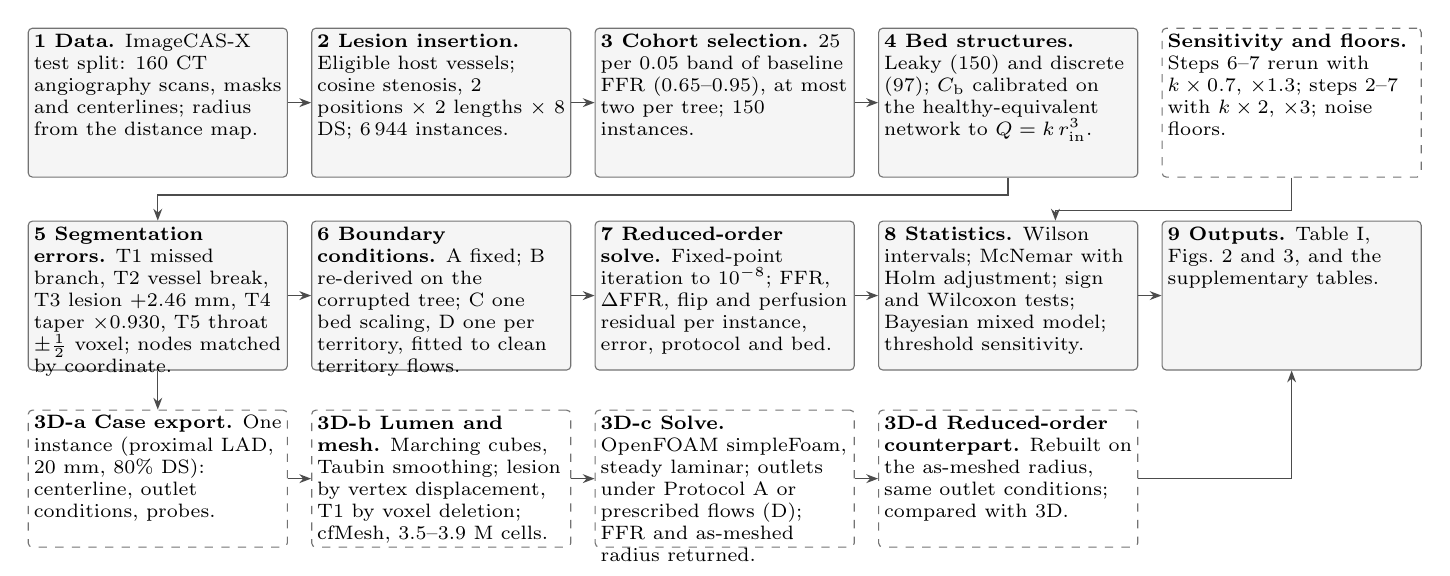
\begin{tikzpicture}[font=\scriptsize, node distance=6mm and 2.6mm,
  box/.style={draw=black!55, fill=black!4, rounded corners=1.5pt, inner sep=2pt, anchor=north west},
  cfd/.style={box, fill=white, dashed},
  arr/.style={-{Stealth[length=1.5mm]}, draw=black!70, line width=0.5pt}]
\def\px{3.6}
\node[box] (data) at (0,0) {\parbox[t][1.75cm][t]{3.15cm}{\raggedright \textbf{1 Data.} \mbox{ImageCAS-X} test split: 160 CT angiography scans, masks and
  centerlines; radius from the distance map.}};
\node[box] (sweep) at (\px,0) {\parbox[t][1.75cm][t]{3.15cm}{\raggedright \textbf{2 Lesion insertion.} Eligible host vessels; cosine stenosis, 2 positions
  $\times$ 2 lengths $\times$ 8 DS; 6\,944 instances.}};
\node[box] (select) at (2*\px,0) {\parbox[t][1.75cm][t]{3.15cm}{\raggedright \textbf{3 Cohort selection.} 25 per 0.05 band of baseline FFR (0.65--0.95), at
  most two per tree; 150 instances.}};
\node[box] (bed) at (3*\px,0) {\parbox[t][1.75cm][t]{3.15cm}{\raggedright \textbf{4 Bed structures.} Leaky (150) and discrete (97); $C_\mathrm{b}$ calibrated on the
  healthy-equivalent network to $Q = k\,r_\mathrm{in}^3$.}};
\node[box, dashed, fill=white] (sens) at (4*\px,0) {\parbox[t][1.75cm][t]{3.15cm}{\raggedright \textbf{Sensitivity and floors.} Steps 6--7 rerun with
  $k \times 0.7$, $\times 1.3$; steps 2--7 with $k \times 2$, $\times 3$; noise floors.}};
\node[box] (err) at (0,-2.45) {\parbox[t][1.75cm][t]{3.15cm}{\raggedright \textbf{5 Segmentation errors.} T1 missed branch, T2 vessel break, T3 lesion
  $+2.46$~mm, T4 taper $\times 0.930$, T5 throat $\pm\tfrac12$ voxel; nodes matched by coordinate.}};
\node[box] (prot) at (\px,-2.45) {\parbox[t][1.75cm][t]{3.15cm}{\raggedright \textbf{6 Boundary conditions.} A fixed; B re-derived on the corrupted tree;
  C one bed scaling, D one per territory, fitted to clean territory flows.}};
\node[box] (solve) at (2*\px,-2.45) {\parbox[t][1.75cm][t]{3.15cm}{\raggedright \textbf{7 Reduced-order solve.} Fixed-point iteration to $10^{-8}$;
  FFR, $\Delta$FFR, flip and perfusion residual per instance, error, protocol and bed.}};
\node[box] (stats) at (3*\px,-2.45) {\parbox[t][1.75cm][t]{3.15cm}{\raggedright \textbf{8 Statistics.} Wilson intervals; McNemar with Holm adjustment; sign
  and Wilcoxon tests; Bayesian mixed model; threshold sensitivity.}};
\node[box] (out) at (4*\px,-2.45) {\parbox[t][1.75cm][t]{3.15cm}{\raggedright \textbf{9 Outputs.} Table I, Figs.~2 and 3, and the supplementary tables.}};
\node[cfd] (exp) at (0,-4.85) {\parbox[t][1.6cm][t]{3.15cm}{\raggedright \textbf{3D-a Case export.} One instance (proximal LAD, 20~mm, 80\% DS): centerline,
  outlet conditions, probes.}};
\node[cfd] (mesh) at (\px,-4.85) {\parbox[t][1.6cm][t]{3.15cm}{\raggedright \textbf{3D-b Lumen and mesh.} Marching cubes, Taubin smoothing; lesion by vertex
  displacement, T1 by voxel deletion; cfMesh, 3.5--3.9~M cells.}};
\node[cfd] (foam) at (2*\px,-4.85) {\parbox[t][1.6cm][t]{3.15cm}{\raggedright \textbf{3D-c Solve.} OpenFOAM simpleFoam, steady laminar; outlets under
  Protocol A or prescribed flows (D); FFR and as-meshed radius returned.}};
\node[cfd] (twin) at (3*\px,-4.85) {\parbox[t][1.6cm][t]{3.15cm}{\raggedright \textbf{3D-d Reduced-order counterpart.} Rebuilt on the as-meshed radius, same outlet
  conditions; compared with 3D.}};
\foreach \u/\v in {data/sweep, sweep/select, select/bed, err/prot, prot/solve, solve/stats, stats/out,
  exp/mesh, mesh/foam, foam/twin} \draw[arr] (\u) -- (\v);
\draw[arr] (bed.south) -- ++(0,-0.22) -| (err.north);
\draw[arr] (sens.south) -- ++(0,-0.42) -| ([xshift=6mm]stats.north);
\draw[arr] (err.south) -- (exp.north);
\draw[arr] (twin.east) -| (out.south);
\end{tikzpicture}
\caption{Analysis pipeline. Shaded boxes: reduced-order arm, run for every
instance. Dashed boxes: sensitivity and noise-floor analyses (top right) and the 3D case study (bottom row), whose
steps 3D-b and 3D-c ran on the CFD machine.}\label{fig:pipeline}
\end{figure}

\FloatBarrier
\Needspace{16\baselineskip}
\section{Exclusions}
Table~\ref{tab:excl} lists every exclusion. Protocols C and D require at least two territories that retain a
vessel. A Protocol C fit at its search bound is a failure (two half-voxel throat-error models; 10 of 4\,940
noise-floor draws). Protocol D fits at the $10^{\pm 3}$ bound keep a defined residual and are retained (two
missed-branch models, residual 0.08 and 0.11; 23 throat-error models with a narrowed throat, most failing the check).
Under Protocol A a vessel break can remove every node with bed outflow (36 discrete, 2 leaky); scored as flips (FFR 1),
these raise the discrete-bed vessel-break flip rate from 40\% to 43\%.
\begin{table}[!ht]
\caption{Cells With Excluded Models}\label{tab:excl}
\centering\footnotesize
\begin{tabular}{@{}lllrl@{}}
\toprule
Bed & Error & Protocol & Solved & Excluded (reason: count)\\
\midrule
\inputtab supplement_tables/tab_exclusions_nz.tex 
\bottomrule
\end{tabular}
\end{table}

\FloatBarrier
\Needspace{16\baselineskip}
\section{Mixed-Effects Model of Flips}
\begin{table}[!ht]
\caption{Bayesian Mixed-Effects Logistic Model of Flips: Posterior Mean Log-Odds (95\% Interval)}\label{tab:glmm}
\centering\footnotesize
\begin{tabular}{@{}lcc@{}}
\toprule
Term & Discrete bed & Leaky bed\\
\midrule
\inputtab supplement_tables/tab_glmm.tex 
\bottomrule
\end{tabular}
\\[3pt]
\parbox{0.85\textwidth}{\footnotesize Reference levels: T1 (missed branch) and Protocol A. Baseline-band terms are
omitted from the table. Random intercepts for patient and lesion slot. The model agrees with the paired tests in direction. Fitted by variational inference; intervals are
posterior mean $\pm 1.96$ posterior standard deviations from the variational approximation.}
\end{table}

\FloatBarrier
\Needspace{16\baselineskip}
\section{Sensitivity Analyses}
\subsection{Perfusion-Check Threshold}
Table~\ref{tab:thr} gives passes-and-wrong at the 10\% threshold and at the 13\% and 16\% sensitivities.
\begin{table}[!ht]
\caption{Proportion of Models That Pass the Perfusion Check and Are Materially Wrong, \% (Wilson 95\% Interval), by
Perfusion-Check Threshold}\label{tab:thr}
\centering\footnotesize
\begin{tabular}{@{}lllrcccrc@{}}
\toprule
 & & & & \multicolumn{3}{c}{Passes and wrong, \% of $n$} & \multicolumn{2}{c}{At 10\%}\\
\cmidrule(lr){5-7}\cmidrule(l){8-9}
Bed & Errors & Protocol & $n$ & 10\% & 13\% & 16\% & Pass & Wrong among passing, \%\\
\midrule
\inputtab supplement_tables/tab_thresholds.tex 
\bottomrule
\end{tabular}
\\[3pt]
\parbox{0.85\textwidth}{\footnotesize Materially wrong: $|\Delta\mathrm{FFR}| > 0.05$. The 13\% and 16\% thresholds were analyzed as sensitivities. $n$ counts models with a
defined perfusion residual: T2 under Protocols A and B in the leaky bed, $n = 100$; T2 under Protocol B in the
discrete bed, $n = 60$. Protocol D matches every territory flow, so its passes-and-wrong proportion equals its
materially wrong proportion.}
\end{table}

\FloatBarrier
\Needspace{16\baselineskip}
\subsection{Hyperemic Demand}\label{sec:demand}
With $k = 562$~s$^{-1}$, a vessel with the normal proximal LAD diameter of 3.7~mm carries 214~mL/min, within one standard deviation of the hyperemic flow measured in that artery by continuous thermodilution ($228 \pm 71$ to $293 \pm 102$~mL/min). The cohort's median demand was 2.28~mL/s (137~mL/min) per tree.
The demand constant $k$ was scaled by 0.7 and 1.3 and the full ablation was repeated with the same cohort
(Table~\ref{tab:demand}). The ordering of topological against caliber errors under fixed boundary conditions, and of
Protocols B and C against Protocol A for the topological errors, was unchanged at both levels in both beds. The taper,
which flipped fewer decisions under Protocol C than under Protocol A at the primary demand, flipped one and two more
at 1.3 times the demand (7 against 6 of 97; 11 against 9 of 150). The magnitudes changed with demand, which moves the
clean FFR of every instance (leaky-bed median 0.869, 0.801 and 0.741 at 0.7, 1.0 and 1.3 times the demand) and
therefore the number of instances near the threshold, as well as the pressure loss across the lesion. The proportion
of tuned topological-error models that pass the perfusion check while materially wrong fell to 3\% in the leaky bed
at 0.7 times the demand, comparable with the simulated floor for correct anatomy (3.9\% at the primary demand); in
the discrete bed it remained between 12\% and 25\%.
\begin{table}[!h]
\caption{Sensitivity to Hyperemic Demand}\label{tab:demand}
\centering\small
\begin{tabular}{@{}llcccccc@{}}
\toprule
Bed & Demand scale & \multicolumn{2}{c}{Flip, \% (Protocol A)} & \multicolumn{2}{c}{Topological flip, \%} &
Passes and wrong, \% & Missed-branch $\Delta$FFR\\
\cmidrule(lr){3-4}\cmidrule(lr){5-6}
 & & Topological & Caliber & B & C & (C, topological) & median, A / C\\
\midrule
Discrete & 0.7 & 32 (25--40) & 6 (3--10) & 12 (8--18) & 18 (12--27) & 12 (7--19) & 0.070 / 0.057 \\
 & 1.0 & 33 (26--41) & 10 (7--15) & 14 (10--20) & 19 (13--28) & 19 (13--28) & 0.095 / 0.077 \\
 & 1.3 & 40 (32--48) & 5 (2--9) & 16 (11--22) & 19 (13--28) & 25 (18--34) & 0.106 / 0.091 \\
Leaky & 0.7 & 20 (16--26) & 6 (4--9) & 7 (4--10) & 9 (5--14) & 3 (1--7) & 0.032 / 0.010 \\
 & 1.0 & 32 (26--38) & 6 (4--9) & 5 (3--8) & 8 (5--13) & 8 (5--13) & 0.047 / 0.015 \\
 & 1.3 & 37 (32--43) & 4 (2--7) & 5 (3--9) & 8 (4--13) & 12 (8--18) & 0.057 / 0.021 \\
\bottomrule
\end{tabular}
\\[3pt]
\parbox{0.9\textwidth}{\footnotesize Demand scale 1.0 is the primary analysis ($k = 562$~s$^{-1}$). Percentages with Wilson 95\%
intervals in parentheses. Missed-branch $\Delta$FFR is over the instances in which Protocol C was defined.}
\end{table}


\FloatBarrier
\Needspace{16\baselineskip}
\subsection{Demand Replication With Re-Selected Cohorts}\label{sec:replication}
The whole pipeline was repeated with $k$ doubled and tripled, with cohorts reselected at that demand. At three times
the demand only 17 instances met the discrete-bed criteria, so the discrete arm is reported at twice the demand
(Table~\ref{tab:repl}). The excess of tuned over re-derived passes-and-wrong at twice the demand was significant in
three of four caliber comparisons and in no topological one.
\begin{table}[!ht]
\caption{Demand Replication: Flip and Passes-and-Wrong Rates, \% (Wilson 95\% Interval)}\label{tab:repl}
\centering\footnotesize\setlength{\tabcolsep}{3pt}
\begin{tabular}{@{}lrrcccccccccc@{}}
\toprule
 & & & \multicolumn{2}{c}{Flip, A} & \multicolumn{2}{c}{Topological flip} & \multicolumn{3}{c}{Topological passes and wrong} & \multicolumn{3}{c}{Caliber passes and wrong}\\
\cmidrule(lr){4-5}\cmidrule(lr){6-7}\cmidrule(lr){8-10}\cmidrule(l){11-13}
Bed & $k$ scale & Inst. & Topol. & Caliber & C & D & B & C & D & B & C & D\\
\midrule
\inputtab supplement_tables/tab_replication.tex 
\bottomrule
\end{tabular}
\\[3pt]
\parbox{0.95\textwidth}{\footnotesize Scale 1 is the primary analysis ($k = 562$~s$^{-1}$, primary cohort). Scales 2 and 3 use
cohorts reselected at that demand. Passes and wrong: perfusion residual below 10\% and $|\Delta\mathrm{FFR}| > 0.05$;
denominators are models with a defined residual, as in Table I of the main text.}
\end{table}

\FloatBarrier
\Needspace{16\baselineskip}
\subsection{Grey Zone}\label{sec:grey}
Flips beyond the grey zone end outside 0.75--0.85 (Table~\ref{tab:grey}); 30\% (discrete) and 33\% (leaky) of clean models lie within.
\begin{table}[!ht]
\caption{Flips and Flips Beyond the Grey Zone (0.75--0.85), \% of Models (Wilson 95\% Interval)}\label{tab:grey}
\centering\footnotesize
\begin{tabular}{@{}llrccrcc@{}}
\toprule
 & & \multicolumn{3}{c}{Topological errors} & \multicolumn{3}{c}{Caliber errors}\\
\cmidrule(lr){3-5}\cmidrule(l){6-8}
Bed & Protocol & $n$ & Flip & Beyond zone & $n$ & Flip & Beyond zone\\
\midrule
\inputtab supplement_tables/tab_greyzone.tex 
\bottomrule
\end{tabular}
\end{table}

\FloatBarrier
\Needspace{16\baselineskip}
\section{Caliber Error at the Stenosis Throat}\label{sec:throat}
The throat error (T5) re-inserts each lesion with its throat diameter changed by half the in-plane voxel size
(spacing median 0.352~mm; throat radius $\pm 0.088$~mm; 7.3 points of DS, 4.5--9.8) or its DS changed by $\pm 10$ points. The $\pm 10$-point magnitude lies within the published CT-versus-invasive disagreement (standard deviation 12.3--12.4 points). Protocol B equals
Protocol A for this error by construction (Table~\ref{tab:throat}). Protocol C fits at the search bound were excluded
(2 at half a voxel, 8 at $\pm 10$ points). The 64 Protocol D fits at the parameter bound, all with an increased
stenosis, were retained; excluding them would raise passes-and-wrong by up to 13 points.
\begin{table}[!ht]
\caption{Throat Caliber Error: Flips, Passes-and-Wrong and Flips Beyond the Grey Zone, \% of Models (Wilson 95\% Interval)}\label{tab:throat}
\centering\footnotesize\setlength{\tabcolsep}{3pt}
\begin{tabular}{@{}llrccc rccc@{}}
\toprule
 & & \multicolumn{4}{c}{Discrete bed (97 instances)} & \multicolumn{4}{c}{Leaky bed (150 instances)}\\
\cmidrule(lr){3-6}\cmidrule(l){7-10}
Error & Protocol & $n$ & Flip & Passes and wrong & Beyond zone & $n$ & Flip & Passes and wrong & Beyond zone\\
\midrule
Throat $-\tfrac12$ voxel & A, B & 97 & 28 (20--37) & 26 (18--35) & 16 (10--25) & 150 & 25 (19--33) & 43 (36--51) & 15 (10--22) \\
 & C & 96 & 30 (22--40) & 49 (39--59) & 23 (16--32) & 149 & 26 (19--33) & 68 (61--75) & 21 (15--28) \\
 & D & 97 & 30 (22--40) & 84 (75--90) & 25 (17--34) & 150 & 27 (21--35) & 91 (85--94) & 19 (14--26) \\
\addlinespace[2pt]
Throat $+\tfrac12$ voxel & A, B & 97 & 32 (24--42) & 32 (24--42) & 12 (7--20) & 150 & 47 (39--55) & 41 (34--49) & 26 (20--34) \\
 & C & 97 & 45 (36--55) & 65 (55--74) & 21 (14--30) & 150 & 49 (41--57) & 69 (61--76) & 38 (31--46) \\
 & D & 97 & 49 (40--59) & 77 (68--85) & 28 (20--37) & 150 & 49 (41--57) & 71 (64--78) & 39 (31--47) \\
\addlinespace[2pt]
$\pm\tfrac12$ voxel pooled & A, B & 194 & 30 (24--37) & 29 (23--36) & 14 (10--20) & 300 & 36 (31--42) & 42 (37--48) & 21 (16--26) \\
 & C & 193 & 38 (31--45) & 57 (50--64) & 22 (17--28) & 299 & 37 (32--43) & 69 (63--74) & 29 (25--35) \\
 & D & 194 & 40 (33--47) & 80 (74--85) & 26 (21--33) & 300 & 38 (33--44) & 81 (76--85) & 29 (24--34) \\
\addlinespace[2pt]
DS $\pm10$ pooled & A, B & 194 & 40 (33--47) & 20 (15--26) & 27 (22--34) & 300 & 42 (37--48) & 40 (34--45) & 35 (30--40) \\
 & C & 187 & 44 (37--52) & 51 (44--58) & 37 (30--44) & 299 & 43 (38--49) & 62 (56--67) & 41 (35--46) \\
 & D & 194 & 45 (38--52) & 75 (68--80) & 40 (34--47) & 300 & 44 (38--49) & 86 (81--89) & 40 (35--46) \\
\bottomrule
\end{tabular}
\\[3pt]
\parbox{0.95\textwidth}{\footnotesize Throat $\mp\tfrac12$ voxel: throat diameter narrowed or widened by half the in-plane voxel size. DS $\pm10$: diameter stenosis raised or lowered by 10 points, both signs pooled. Passes and wrong: perfusion residual below 10\% and $|\Delta\mathrm{FFR}| > 0.05$. Beyond zone: flips whose corrupted FFR lies outside 0.75--0.85. Protocols A and B coincide for throat errors. Protocol C fits on the search bound are excluded, which reduces $n$. For comparison, topological errors under Protocol A flipped 33\% (26--41\%) and 32\% (26--38\%) of models and caliber errors away from the throat 10\% (7--15\%) and 6\% (4--9\%).}
\end{table}

\FloatBarrier
\Needspace{16\baselineskip}
\section{Territory Granularity}\label{sec:granularity}
Protocols C and D were repeated with each main-branch territory divided again at its first bifurcation (median four territories, discrete; five, leaky). A territory without a surviving vessel entered the residual as a 100\% mismatch; without this rule, discrete topological passes-and-wrong would have risen to 26\%. With the main-branch partition the
procedure reproduced the original results exactly (Table~\ref{tab:gran}). Throat-error models removed from the count
all failed the finer check; none had its FFR corrected, and 76--88\% of tuned throat-error models that passed remained
materially wrong. Flip rates changed by at most five models per cell. The simulated noise floor was computed at
main-branch level only.
\begin{table}[!ht]
\caption{Passes and Wrong, \% (Wilson 95\% Interval), at Main-Branch and Finer Territory Level}\label{tab:gran}
\centering\footnotesize
\begin{tabular}{@{}lllrccc@{}}
\toprule
Bed & Errors & Protocol & $n$ & Main branch & Finer & $p$\\
\midrule
Discrete & T1+T2 & C & 104 & 19 (13--28) & 7 (3--13) & $<0.001$ \\
 & & D & 104 & 20 (14--29) & 3 (1--8) & $<0.001$ \\
 & T3+T4 & C & 194 & 5 (2--9) & 5 (3--9) & 1.0 \\
 & & D & 194 & 18 (13--24) & 23 (18--30) & 0.002 \\
 & T5, $\pm\tfrac12$ voxel & A, B & 194 & 29 (23--36) & 25 (20--32) & 0.016 \\
 & & C & 193 & 57 (50--64) & 51 (44--58) & 0.003 \\
 & & D & 194 & 80 (74--85) & 78 (71--83) & 0.12 \\
\addlinespace[2pt]
Leaky & T1+T2 & C & 171 & 8 (5--13) & 5 (2--9) & 0.07 \\
 & & D & 171 & 5 (3--10) & 2 (1--6) & 0.18 \\
 & T3+T4 & C & 300 & 12 (9--17) & 12 (9--17) & 1.0 \\
 & & D & 300 & 4 (2--7) & 9 (7--13) & $<0.001$ \\
 & T5, $\pm\tfrac12$ voxel & A, B & 300 & 42 (37--48) & 35 (30--41) & $<0.001$ \\
 & & C & 299 & 69 (63--74) & 60 (55--66) & $<0.001$ \\
 & & D & 300 & 81 (76--85) & 81 (76--85) & 1.0 \\
\bottomrule
\end{tabular}
\\[3pt]
\parbox{0.85\textwidth}{\footnotesize Passes and wrong: perfusion residual below 10\% and $|\Delta\mathrm{FFR}| > 0.05$. Main branch: subtrees below each child of the first bifurcation (two or three per tree). Finer: each divided again at its own first bifurcation (median four, discrete; five, leaky). $n$ counts models with a defined residual at both levels; Protocol C fits on the search bound at either level are excluded. For throat errors the FFR of Protocols A and B is the same at both levels and only the residual changes. $p$: exact McNemar test, paired by model.}
\end{table}

\FloatBarrier
\Needspace{16\baselineskip}
\section{Overlap and Topology of the Corrupted Trees}\label{sec:overlap}
Each tree was represented as cylinders of node radius and element length (a tube model) and compared with its clean
tree; no error changed the number of connected components (Table~\ref{tab:overlap}). Of the topological errors that
changed the decision, 91\% (79--96\%, discrete) and 62\% (51--72\%, leaky) kept a whole-scan DSC at or above the
inter-observer 0.928. The AUC of tree DSC for a Protocol A flip was 0.65 (discrete) and 0.79 (leaky) across error
types and 0.54 and 0.70 within topological errors. The taper DSC exceeds 0.928 because it narrows only the tree beyond
the lesion (median 40\% of its volume).
\begin{table}[!ht]
\caption{Tube-Model Overlap of Corrupted Trees, Median (IQR), and Protocol A Decision Changes}\label{tab:overlap}
\centering\footnotesize
\begin{tabular}{@{}llrcccrc@{}}
\toprule
Bed & Error & $n$ & DSC, tree & DSC, scan & clDice & Flow lost, \% & Flip A, \% \\
\midrule
Discrete & T1 & 77 & 0.975 (0.947--0.984) & 0.985 (0.977--0.991) & 0.940 (0.903--0.963) & 27 (14--43) & 27 (19--38) \\
 & T2 & 96 & 0.893 (0.701--0.937) & 0.935 (0.888--0.960) & 0.847 (0.544--0.907) & 30 (15--100) & 40 (29--53)$^a$ \\
 & T3 & 97 & 0.996 (0.995--0.997) & 0.998 (0.998--0.998) & 1.000 & 0 & 7 (4--14) \\
 & T4 & 97 & 0.971 (0.947--0.981) & 0.983 (0.974--0.989) & 1.000 & 0 & 13 (8--22) \\
Leaky & T1 & 118 & 0.969 (0.946--0.980) & 0.983 (0.975--0.990) & 0.930 (0.899--0.957) & 9 (6--17) & 18 (12--26) \\
 & T2 & 149 & 0.895 (0.721--0.936) & 0.934 (0.886--0.962) & 0.855 (0.517--0.899) & 14 (7--56) & 43 (35--51) \\
 & T3 & 150 & 0.997 (0.995--0.998) & 0.998 (0.998--0.999) & 1.000 & 0 & 2 (1--6) \\
 & T4 & 150 & 0.972 (0.951--0.981) & 0.983 (0.976--0.988) & 1.000 & 0 & 9 (6--15) \\
\midrule
\multicolumn{3}{@{}l}{T2, right coronary artery} & 0.62--0.63 & 0.85--0.86 & 0.45--0.49 & & \\
\bottomrule
\end{tabular}
\\[3pt]
\parbox{0.85\textwidth}{\footnotesize Flip A: Wilson 95\% interval. Flow lost: share of the clean model's bed outflow on deleted nodes. $^a$ $n = 60$; right coronary breaks leave no discrete outlet under Protocol A.}
\end{table}

\FloatBarrier
\Needspace{16\baselineskip}
\section{Detection Before and During Tuning}\label{sec:detector}
Positives are error models; negatives are the correct-anatomy draws of the simulated floor before tuning
(Table~\ref{tab:detector}). Correct anatomy without noise has a residual below $10^{-8}$; with noise its median is
0.10. With the error models' targets carrying the same noise, the AUC for topological errors was 0.82 (discrete) and
0.56 (leaky).
\begin{table}[!ht]
\caption{Detection Before and During Tuning Against Correct Anatomy With Noisy Targets}\label{tab:detector}
\centering\footnotesize\setlength{\tabcolsep}{4pt}
\begin{tabular}{@{}lllrccccc@{}}
\toprule
Bed & Quantity & Positives & $n$ & AUC & Sens.\ at 0.10, \% & FA at 0.10, \% & 5\% FA value & Sens.\ at 5\% FA, \%\\
\midrule
Discrete & Pre-tuning residual & Topological & 137 & 0.77 (0.71--0.82) & 83 (76--89) & 48 & 0.22 & 47 (39--55) \\
 &  & Flip under B$^a$ & 36 & 0.57 (0.46--0.69) & 69 (53--82) & 48 & 0.22 & 22 (12--38) \\
 & $|\ln C|$ & Topological & 104 & 0.47 (0.40--0.53) & 30 (22--39) & 37 & 0.24 & 9 (5--16) \\
 &  & Flip or P\&W under C$^a$ & 61 & 0.53 (0.44--0.62) & 41 (30--54) & 37 & 0.24 & 15 (8--26) \\
\addlinespace[2pt]
Leaky & Pre-tuning residual & Topological & 218 & 0.22 (0.18--0.27) & 19 (15--25) & 50 & 0.23 & 6 (3--9) \\
 &  & Flip under B$^a$ & 16 & 0.21 (0.08--0.36) & 12 (3--36) & 50 & 0.23 & 6 (1--28) \\
 & $|\ln C|$ & Topological & 171 & 0.12 (0.09--0.15) & 3 (1--7) & 34 & 0.24 & 2 (1--5) \\
 &  & Flip or P\&W under C$^a$ & 66 & 0.66 (0.55--0.77) & 61 (49--71) & 34 & 0.24 & 59 (47--70) \\
\bottomrule
\end{tabular}
\\[3pt]
\parbox{0.9\textwidth}{\footnotesize Negatives: 1\,940 (discrete) and 3\,000 (leaky; 2\,990 for $|\ln C|$) correct-anatomy draws on 97 and 150 instances. FA, false alarm; P\&W, passes and wrong; Sens., sensitivity. $^a$Any error type.}
\end{table}

\FloatBarrier
\Needspace{16\baselineskip}
\section{Noise Floors}\label{sec:floor}
The perfusion-check bound is $1.96 \times (10\text{--}15\%) \approx 20$--29\% for one model output against one
measurement, from the within-subject variation of hyperemic myocardial blood flow. The repeat-measurement floor uses
the test--retest standard deviation of invasive FFR, 0.018 (5.0--6.5\% across cells). The simulated floor perturbs,
in 20 draws per instance, cardiac output (relative standard deviation 0.05), aortic pressure (0.056), viscosity (0.02),
territory flow shares (0.10) and the measured territory flows (0.083), then tunes as in Protocol C
(Table~\ref{tab:floor}).
\begin{table}[!ht]
\caption{Simulated Floor: Correct Anatomy Tuned to Noisy Perfusion}\label{tab:floor}
\centering\footnotesize
\begin{tabular}{@{}lrrcccrc@{}}
\toprule
Bed & Instances & Draws solved & Flip, \% & Median $|\Delta$FFR$|$ & 95th pct. $|\Delta$FFR$|$ & Pass, \% &
Pass and wrong, \%\\
\midrule
\inputtab supplement_tables/tab_floor.tex 
\bottomrule
\end{tabular}
\end{table}

\FloatBarrier
\Needspace{16\baselineskip}
\section{Three-Dimensional Case Study: Mesh Checks}\label{sec:cfd}
Surfaces were extracted by marching cubes with Taubin smoothing; meshes of 3.5--3.9 million cells (cfMesh) had
25~\textmu m cells within $\pm 4$~mm of the throat and four boundary layers. OpenFOAM simpleFoam (ESI v2406; SIMPLE;
bounded second-order upwind) ran 3\,000 iterations per solve to scaled residuals below $10^{-5}$. A finer throat zone
raised the baseline FFR by 0.0019--0.0021, above the idealized-case discretization uncertainty of $5.5\times10^{-4}$,
so the patient-case uncertainty is about 0.002, against an error effect of 0.074. The finest mesh missed the strict residual limit (velocity residual $1.08\times10^{-5}$) with a steady inlet pressure (Table~\ref{tab:d7}). All 3D-to-0D
comparisons use a reduced-order counterpart rebuilt on the meshed radius.
\begin{table}[!ht]
\caption{Throat-Zone Resolution Test, Baseline Lumen. The 8.31~M-cell mesh did not meet the strict residual limit at
3\,000 iterations (see text).}\label{tab:d7}
\centering\footnotesize
\begin{tabular}{@{}lrrrrr@{}}
\toprule
Mesh & Cells (M) & FFR & $\Delta$FFR & Outlet flow change, \% & Flagged cell to throat, mm\\
\midrule
\inputtab supplement_tables/tab_d7.tex 
\bottomrule
\end{tabular}
\end{table}

\end{document}
